%!TEX encoding = UTF-8 Unicode
%!TEX root = ../labs.tex

\Lab{\LabWeekFOUR}
\begin{Goals}
%!TEX encoding = UTF-8 Unicode
%!TEX root = ../labs.tex

\item Kunna skapa singelobjekt med medlemmar.
\item Förstå kvalificerade namn och import.
\item Förstå synlighet och skuggning.
\item Kunna använda tupler.
\item Kunna använda uppdelade parameterlistor.

\end{Goals}

\begin{Preparations}
\item Gör övning \texttt{\ExeWeekFOUR} och repetera övning \texttt{\ExeWeekTHREE}.
\item Repetera appendix~\ref{appendix:terminal}, ~\ref{appendix:compile}, och ~\ref{appendix:debug}.
\end{Preparations}



\subsection{Bakgrund}


\begin{minipage}{0.48\textwidth}
\begin{figure}[H]
  \centering
  
\includegraphics[width=\textwidth]{../img/blockmole-sky-grass.png}
%  \caption{En lundensisk blockmullvad fångad på bild under aktivt grävanade.}
  \label{lab:blockmole:fig:mole}
\end{figure}
\end{minipage}%
%
\hfill\begin{minipage}{0.45\textwidth}
\noindent\textbf{Blockmullvad} (\textit{Talpa laterculus}) är ett fantasidjur i familjen mullvadsdjur.
Den är känd för sitt karaktäristiska kvadratiska utseende.
Den lever mest ensam i sina underjordiska gångar som, till skillnad från den verkliga mullvadens (\emph{Talpa europaea}) gångar, har helt raka väggar.
\end{minipage}



\subsection{Obligatoriska uppgifter}


\Task \emph{Skapa katalog och kodfil.}
Du ska, steg för steg, skapa ett program som låter användaren interagera med en levande blockmullvad. Använd en editor, t.ex. \texttt{atom}, kompilera ditt program i terminalen med \texttt{scalac} och kör med \texttt{scala}.

\Subtask
Skapa en ny fil med namnet \texttt{blockmole.scala} i en ny katalog i din hemkatalog, till exempel \texttt{\textasciitilde/pgk/w04/lab/blockmole.scala}, där \texttt{\textasciitilde} är din hemkatalog.
\begin{REPLnonum}
> mkdir -p ~/pgk/w04/lab
> atom ~/pgk/w04/lab/blockmole.scala
\end{REPLnonum}


\Subtask
Navigera till din nya katalog och kontrollera att din nya fil finns där.
\begin{REPLnonum}
> cd ~/pgk/w04/lab/
> ls
blockmole.scala
\end{REPLnonum}

\Subtask
Gör en paketdeklaration i början av filen \code{blockmole.scala} så att koden du ska skriva nedan ingår i paketet \code{blockmole}.

\Subtask
Deklarera sedan ett singelobjekt med namnet \code{Main} med en \code{main}-procedur som skriver ut texten: \texttt{"Keep on digging!"}

\Subtask
Kompilera ditt program. Kontrollera med \texttt{ls}-kommandot att några filer som slutar på \texttt{class} har skapats i subkatalogen \code{blockmole}. \Pen Varför hamnade bytekoden i denna katalog?

\Subtask
Kör kommandot \texttt{scala blockmole.Main} för att exekvera ditt program och kontrollera utskriften i terminalfönstret.

\vspace{1em}\noindent Nu har du skrivit ett program som uppmanar en blockmullvad att fortsätta gräva. Det programmet är inte så användbart, eftersom mullvadar inte kan inte läsa. Nästa steg är därför att skriva ett grafiskt program.%, snarare än ett textbaserat.



\Task \emph{Skapa en grundstruktur för programmet.}
I mindre program fungerar det bra att samla alla funktioner i ett singelobjekt, men i stora program blir det lättare att hitta i koden och förstå vad den gör om man har flera moduler med olika ansvar. Ditt program ska ha följande övergripande struktur:

\begin{Code}
package blockmole

object Color {
  // Skapar olika färger som behövs i övriga moduler
}

object BlockWindow {
  // Har ett introprog.PixelWindow och ritar blockgrafik
}

object Mole { // Representerar en blockmullvad som kan gräva
  def dig(): Unit = println("Här ska det grävas!")
}

object Main {
  def drawWorld(): Unit = println("Ska rita ut underjorden!")

  def main(args: Array[String]): Unit = {
    drawWorld()
    Mole.dig()
  }
}
\end{Code}

\noindent Skapa programskelettet ovan i filen \code{blockmole.scala} och se till att koden kompilerar utan fel och går att köra med utskrifter som förväntat.

Vi lägger i denna laboration alla moduler i samma fil, men i andra situationer när  modulerna blir stora och/eller ska återanvändas av flera olika program är det bra att ha dem i olika filer så att de kan kompileras och testas separat.


\Task \emph{Lägg till färger i färgmodulen.} I singelobjektet \code{Color} ska vi skapa färger med hjälp av Java-klassen \code{java.awt.Color}. Eftersom vårt singelobjektnamn ''krockar'' med namnet på Java-färgklassen så byter vi namn på Java-klassen till \code{JColor} i importdeklarationen.

\Subtask
Lägg in en importdeklaration med namnbytet direkt efter paketdeklarationen. Vi lägger importen så att den syns i hela paketet eftersom flera objekt behöver tillgång till \code{JColor}. Säkerställ att koden fortfarande kompilerar utan fel.

\Subtask
Skapa sedan nedan färger i objektet \code{Color}:
\begin{Code}
object Color {
  val black  = new JColor(  0,   0,   0)
  val mole   = new JColor( 51,  51,   0)
  val soil   = new JColor(153, 102,  51)
  val tunnel = new JColor(204, 153, 102)
}
\end{Code}


\Task \emph{Skapa ett ritfönster i modulen för blockgrafik.} Lägg till nedan tre variabler i singelobjektet \code{BlockWindow}:

\begin{Code}
  val windowSize = (30, 50)  // (width, height) in number of blocks
  val blockSize  = 10        // number of pixels per block

  val window = new PixelWindow(???, ???, ???)
\end{Code}

\begin{itemize}%[noitemsep]
  \item Importera \code{introprog.PixelWindow} lokalt i \code{BlockWindow}. (En lokal import-deklaration i är bra här eftersom det bara är detta objekt som behöver tillgång till \code{PixelWindow}.)
  \item Gör så att storleken på \code{window} motsvarar blockstorleken gånger bredd resp. höjd i \code{windowSize}.
  \item Ge fönstret en lämplig titel, t.ex. \code{"Digging Blockmole"}.
  \item När du kompilerar behöver du se till att \code{introprog} finns tillgänglig på \code{classpath} (se övning \texttt{\ExeWeekFOUR}).
  \item Om du glömt ordningen på parametrarna till klassen \code{PixelWindow} så kolla i dokumentationen för \code{PixelWindow} \footnote{\url{http://cs.lth.se/pgk/api/}}. Använd namngivna argument vid skapandet av fönstret. Tycker du att koden mer läsbar med namngivna argument? \footnote{Det går tyvärr inte att använda namngivna argument när man instansierar Java-klasser i Scala, men PixelWindow är implementerad i Scala så här fungerar det fint.}
\end{itemize}

För att testa fönstret, lägg till en enkel testritning genom att i proceduren \code{drawWorld} använda \code{BlockWindow.window}, till exempel:
\begin{Code}
  def drawWorld(): Unit = {
    BlockWindow.window.line(100, 10, 200, 20)
  }
\end{Code}
Kompilera och kör och säkerställ att allt fungerar som förväntat.


\Task \emph{Skapa procedur för blockgrafik.} Nu har du gjort ett grafiskt program, men ännu syns ingen mullvad.
Det är dags att skapa koordinatsystemet i blockmullvadens blockvärld.

\Subtask\Pen
Säkerställ att du kan förklara hur koordinaterna i ett \code{PixelWindow} tolkas, genom att med papper och penna rita en enkel skiss av ungefär var positionerna $(0,0)$, $(300, 0)$, $(0, 300)$ och $(300, 300)$ ligger i ett fönster som är 300 bildpunkter brett och 500 bildpunkter högt.

\Subtask
Koordinatsystem i \code{BlockWindow} ska ha kvadratiska, \emph{stora} bildpunkter som består av många fönsterpixlar. Vi kallar dessa stora bildpunkter för \emph{block} för att lättare skilja dem från de enpixelstora bildpunkterna i \code{PixelWindow}. I block-koordinatsystemet för \code{BlockWindow} gäller följande:

\begin{framed}
\noindent \emph{Blockstorleken} anger sidan i kvadraten för ett block räknat i antalet pixlar. Om blockstorleken är $b$, så ligger koordinaten $(x, y)$ i \code{BlockWindow} på koordinaten $(bx, by)$ i \code{PixelWindow}.

\end{framed}

\noindent Implementera funktionen \code{block} i modulen \code{BlockWindow} enligt nedan, så att en kvadrat ritas ut när proceduren anropas. Parametern \code{point} anger block-koordinaten och parametern \code{color} anger färgen. Typ-alias-deklarationen av \code{Pos} ger ett beskrivande typnamn för en 2-tupel av heltal, som vi kan använda i parameterlistor för att betecknande positioner i ett \code{BlockWindow}. Se dokumentationen av \code{fill}-metoden i \code{PixelWindow}. Fyll i det som saknas nedan.
\begin{Code}
  type Pos = (Int, Int)

  def block(pos: Pos)(color: JColor = JColor.gray): Unit = {
    val x = ???
    val y = ???
    window.fill(???)
  }
\end{Code}
Säkerställ att koden kompilerar utan fel.

% %%% Borttagen fråga, då vi använder fill istf att rita en massa linjer som man redan gjort på övningen
% \Subtask\Pen
% Metoden \code{block} ska rita ett antal linjer.
% Hur många linjer ritas ut?
% I vilken ordning ritas linjerna?
% Skriv ner dina svar inför redovisningen.

\Subtask
För att testa din procedur, anropa funktionen \code{BlockWindow.block} några gånger i \code{Main.drawWorld}, dels med utelämnat defaultargument, dels med olika färger ur färgmodulen. Kompilera och kör ditt program och kontrollera att allt fungerar som det ska.



\Task \emph{Skapa rektangelprocedur och underjorden.} Du ska nu skriva en procedur med namnet \code{rectangle} som ritar en rektangel med hjälp av proceduren \code{block}. Sen ska du använda \code{rectangle} i \code{Main.drawWorld} för att rita upp mullvadens underjordiska värld.

\Subtask
Lägg till proceduren \code{rectangle} i grafikmodulen. Procedurhuvudet ska ha följande parametrar uppdelade i tre olika paramterlistor:
\begin{Code}
(leftTop: Pos)(size: (Int, Int))(color: JColor = JColor.gray)
\end{Code}

Parametern \code{leftTop} anger blockkoordinaten för rektangelns övre vänstra hörn och \code{size} anger \code{(bredd, höjd)}.

Använd denna nästlade repetition för att rita ut rektangeln:

\begin{Code}
for (y <- ???) {
	for (x <- ???) {
		block(x, y)(color)
	}
}
\end{Code}

\Subtask\Pen
I vilken ordning ritas blocken i rektangeln ut (lodrät eller vågrät)? Om du är osäker kan du lägga in en utskrift av \code{(x, y)} i den innersta loopen för att se ordningen.

\Subtask\Pen En annan lösning är att i stället anropa \code{fill}-metoden i \code{PixelWindow} direkt för att rita en motsvarande stor rektangel \emph{utan} nästlad loop. Vilka argument ska \code{fill}-anropet då ha?

\Subtask Ändra i \code{Main.drawWorld} så att den ritar ut underjorden, det vill säga en massa jord där blockmullvaden kan gräva sina tunnlar.
 Underjorden ska bestå av en rektangel med färgen \code{Color.soil} som precis täcker fönstret.

Eftersom funktionen \code{rectangle} har mer än en parameter med samma typ som lätt kan blandas ihop utan att kompilatorn hittar felet, ska du namnge det andra argumentet \code{size} vid anropet. För det första argumentet (\code{leftTop}) ska du utnyttja att det går att skippa tupelparenteserna (gäller vid parameterlista med endast en parameter av tupeltyp).

\Subtask Anropa \code{Main.drawWorld} i \code{Mole.main} och testa så att det fungerar.

\Task
I \code{PixelWindow} finns funktioner för att känna av tangenttryckningar och musklick.
Du ska använda de funktionerna för att styra en blockmullvad. Studera dokumentationen för \code{awaitEvent} och \code{Event} i \code{PixelWindow}, samt koden i exempelprogrammet \code{TestPixelWindow} i paketet \code{introprog.examples}.

\Subtask
Lägg till denna funktion i \code{BlockWindow}:
\begin{Code}
  val maxWaitMillis = 10

  def waitForKey(): String = {
    window.awaitEvent(maxWaitMillis)
    while (window.lastEventType != PixelWindow.Event.KeyPressed) {
      window.awaitEvent(maxWaitMillis) // skip other events
    }
    println(s"KeyPressed: " + window.lastKey)
    window.lastKey
  }
\end{Code}
\noindent Det finns olika sorters händelser som ett \code{PixelWindow} kan reagera på, till exempel tangenttryckningar och musklick.
Funktionen som du precis lagt in väntar på en händelse i ditt \code{PixelWindow} med hjälp av (\code{window.awaitEvent}) ända tills det kommer en tangenttryckning (\code{KEY_EVENT}).
När det kommit en tangenttryckning anropas \code{window.lastKey} för att ta reda på vilken bokstav eller vilket tecken det blev, och det resultatet blir också resultatet av \code{waitForKey}, eftersom det ligger sist i blocket.

\Subtask
Utöka proceduren \code{Mole.dig} enligt nedan:
\begin{Code}
  def dig(): Unit = {
    var x = BlockWindow.windowSize._1 / 2
    var y = BlockWindow.windowSize._2 / 2
    var quit = false
    while (!quit) {
      BlockWindow.block(x, y)(Color.mole)
      val key = BlockWindow.waitForKey()
      if      (key == "w") ???
      else if (key == "a") ???
      else if (key == "s") ???
      else if (key == "d") ???
      else if (key == "q") quit = true
    }
  }
\end{Code}

\Subtask Fyll i alla \code{???} så att \code{'w'} styr mullvaden ett steg uppåt, \code{'a'} ett steg åt vänster, \code{'s'} ett steg nedåt och \code{'d'} ett steg åt höger.

\Subtask Kontrollera så att \code{main} bara innehåller två anrop: ett till \code{drawWorld} och ett till \code{dig}. Kompilera och kör ditt program för att se om programmet reagerar på tangenterna w, a, s och d.

\Subtask Om programmet fungerar kommer det bli många mullvadar som tillsammans bildar en lång mask, och det är ju lite underligt. Lägg till ett anrop i \code{Mole.dig} som ritar ut en bit tunnel på position $(x, y)$ efter anropet till \code{BlockWindow.waitForKey} men innan \code{if}-satserna. Kompilera och kör ditt program för att gräva tunnlar med din blockmullvad.

\subsection{Kontrollfrågor}\Checkpoint

\noindent Repetera teorin för denna vecka och var beredd på att kunna svara på dessa frågor när det blir din tur att redovisa vad du gjort under laborationen:

\begin{enumerate}[noitemsep]
\item Till vad används \emph{classpath}?
\item Vad är en \code{jar}-fil?
\item Vad innebär punktnotation?
\item Ge exempel på användning av \code{import} och förklara vad som händer.
\item Vad är fördelen med skuggning och lokala namn?
\item Vi använde flera singelobjekt som olika s.k. \code{moduler} i denna laboration. Vad är fördelen med att att dela upp koden i moduler?
\item Gå igenom målen med laborationen och kontrollera så du har uppfyllt dem.
\end{enumerate}




%\clearpage

\subsection{Frivilliga extrauppgifter}

\Task
Mullvaden kan för tillfället gräva sig utanför fönstret.
Lägg till några \code{if}-satser i början av \code{while}-satsen som upptäcker om \code{x} eller \code{y} ligger utanför fönstrets kant och flyttar i så fall tillbaka mullvaden precis innanför kanten.

\Task
Mullvadar är inte så intresserade av livet ovanför jord, men det kan vara trevligt att se hur långt ner mullvaden grävt sig.
Lägg till en himmelsfärg och en gräsfärg i objektet \code{Color} och rita ut himmel och gräs i \code{Mole.drawWorld}.
Justera också det du gjorde i föregående uppgift, så att mullvaden håller sig under jord. \emph{Tips:} Du har nytta av en interaktiv färgväljare som du kan få genom att anropa \code{introprog.Dialog.selectColor()} i Scala REPL.

\Task
Ändra så att mullvaden kan springa uppe på gräset också, men se till så att ingen tunnel ritas ut där.

\Task
Låt mullvaden fortsätta gräva även om man inte trycker ned någon tangent. Tangenttryckning ska ändra riktningen.

\Subtask
Skapa en ny metod \code{BlockWindow.waitForKeyNonBlocking} som möjliggör tangentbordsavläsning som ej blockerar exekveringen enligt nedan:

\begin{Code}
  def waitForKeyNonBlocking(): String  = {
    import PixelWindow.Event.{KeyPressed, Undefined}

    window.awaitEvent(maxWaitMillis)
    while (window.lastEventType != KeyPressed  &&
           window.lastEventType != Undefined) {
      window.awaitEvent(maxWaitMillis)
    }
    if (window.lastEventType == KeyPressed) window.lastKey else ""
  }
\end{Code}

\Subtask
Lägg till en ny metod \code{BlockWindow.delay} som ska göra det möjligt att hindra blockmullvaden från att springa alltför fort:
\begin{Code}
  def delay(millis: Int): Unit = Thread.sleep(millis)
\end{Code}


\Subtask
Skapa en ny metod \code{BlockWindow.keepOnDigging} som från början är en kopia av metoden \code{dig}. Gör följande tillägg/ändringar:
\begin{enumerate}[nolistsep,noitemsep]

\item Lägg till två variabler \code{var dx} och \code{var dy} i början, som ska hålla reda på riktningen som blockmullvaden gräver. Initialisera dem till \code{0} respektive {1}.

\item Lägg in en fördröjning på 200 millisekunder i den oändliga loopen. Deklarera en konstant \code{delayMillis} på lämpligt ställe i \code{Mole} och använd denna konstant som argument till \code{delay}.

\item Anropa \code{waitForKeyNonBlocking} i stället för \code{waitForKey} och kolla efter knapptryckning enligt nedan kodskelett. Fyll i de saknade delarna så att blockmullvaden rör sig ett steg i rätt riktning i varje looprunda.
\begin{Code}
      if      (key == 'w') { dy = -1; dx = 0 }
      else if (key == 'a') { ??? }
      else if (key == 's') { ??? }
      else if (key == 'd') { ??? }
      else if (key == "q") { quit = true }
      y += ???
      x += ???
\end{Code}

%\item Anpassa fördröjningen efter din förmåga att hinna styra blockmullvaden.

% \item Lägg till så att man kan pausa grävandet om man trycker på blankstegstangenten.
%
% \item Gör så att om man ger en parameter \code{--non-blocking} till programmet när man startar det kan välja mellan om \code{main} anropar \code{dig} eller \code{keepOnDigging}.

\end{enumerate}

\Task\label{lab:blockmole:task:blockworm} \emph{Fånga blockmasken.}


{\raggedright
\begin{minipage}{0.27\textwidth}
\begin{figure}[H]%
  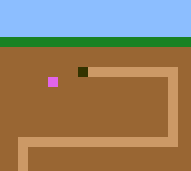
\includegraphics[width=\textwidth]{../img/blockworm.png}
  \label{lab:blockmole:fig:worm}
\end{figure}
\end{minipage}%
}%
\hfill\begin{minipage}{0.69\textwidth}
\noindent\textbf{Blockmask} (\textit{Lumbricus quadratus}) är ett fantasidjur i familjen daggmaskar. Den är känd för att kunna teleportera sig från en plats till en annan på ett ögonblick och är därför svårfångad. Den har i likhet med den verkliga daggmasken (\emph{Lumbricus terrestris}) RGB-färgen $(225, 100, 235)$, men är kvadratisk och exakt ett block stor. Blockmasken är ett eftertraktat villebråd bland blockmullvadar.

\end{minipage}



\Subtask Lägg till modulen \code{Worm} nedan i din kod och använd procedurerna i \code{keepOnDigging} så att blockmullvaden får en blockmask att jaga.


%\begin{figure}
\begin{Code}
object Worm {
  import BlockWindow.Pos

  def nextRandomPos(): Pos = {
    import scala.util.Random.nextInt
    val x = nextInt(BlockWindow.windowSize._1)
    val y = nextInt(BlockWindow.windowSize._2 - 7) + 7
    (x, y)
  }

  var pos = nextRandomPos()

  def isHere(p: Pos): Boolean = pos == p

  def draw(): Unit  = BlockWindow.block(pos)(Color.worm)

  def erase(): Unit = BlockWindow.block(pos)(Color.soil)

  val teleportProbability = 0.02

  def randomTeleport(notHere: Pos): Unit =
    if (math.random < Worm.teleportProbability) {
      erase()
      do pos = nextRandomPos() while (pos == notHere)
      draw()
    }
}
\end{Code}
%\end{figure}

\Subtask Koden i \code{Worm} förutsätter att himmel finns i fönstrets översta $7$ block. Hur många block som är himmel kan egentligen med fördel vara en konstant med ett bra namn på en bra plats. Denna konstant bör användas även i \code{drawWorld}. Fixa det!

\Subtask Gör så att texten \code{"WORM CAUGHT!"} skrivs ut i terminalen om blockmullvaden är på samma plats som blockmasken.

\Subtask Använd parametern \code{notHere} till att förhindra att blockmasken teleporterar sig till samma plats som blockmullvaden.

\Subtask Gör så att blockmullvaden får $1000$ poäng varje gång den fångar blockmasken.

\Subtask Gör så att spelet varar en bestämd, lagom lång tid, innan \code{Game Over}. Använd \code{System.currentTimeMillis} som ger aktuella antalet millisekunder sedan den förste januari 1970. När spelet är slut ska den totala poängen som blockmullvaden samlat skrivas ut i terminalen.

\Subtask Gör så att spelets hastighet ökar (d.v.s. att fördröjningen i spel-loopen minskar) efter en viss tid. I samband med det ska sannolikheten för att blockmasken teleporterar sig öka.

\Task
Skriv om iterationerna i \code{waitForKey} och \code{waitForKeyNonBlocking} så att de använder \code{do while} i stället. Vilken variant tycker du är lättast att förstå?
